This chapter outline the fundamental theories behind flapping-based propulsion used in aquatic creatures, described in \ref{sec:6} and also optimisation method used in optimisation process in flapping fin panel case, described in \ref{sec:11}.
\section{Fundamentals of Flapping-based Propulsion}
\label{sec:6}
This subsection will explain the fundamentals of flapping motion on thrust generation. Basic terminology and kinematics of caudal fin are outlined in \ref{sec:7}, Navier-Stokes equation applied in flapping fin is derived in \ref{sec:8}, relevant scaling parameters are introduced in \ref{sec:9}, and finally caudal fin effect on surrounding water is discussed in \ref{sec:10}.
\subsection{Terminology and Kinematics of Caudal Fin}
\label{sec:7}
Terminologies of caudal fin are introduced first before formulating the kinematics of caudal fin. Following \citet{sfakiotakis}, relevant geometrical properties in caudal fin is outlined as follows: fin span, denoted by $b$ refers to the straight line connecting one tip of the fin to the other tip, chord length $c$ is the length of a straight line that goes from the trailing edge to the leading edge of the fin, pitching length $d$ refers to the straight line from trailing edge to the pitching axis, swept back angle $\Lambda$ is the angle of leading edge with respect to it's symmetrical axis, and surface area $S_{c}$ is the projected fin area. Figure \ref{fig:caudalfinview} illustrated the caudal fin from lateral perspective.
\begin{figure}[H]
    \centering
    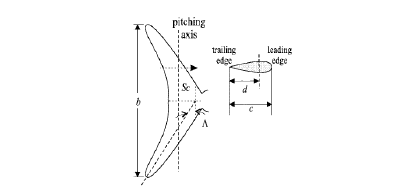
\includegraphics[scale=0.75]{caudalfinview.png}
    \caption{Lateral view of caudal fin. Adapted from \cite{magnuson}}
    \label{fig:caudalfinview}
\end{figure}
Fish swims by exerting force against the surrounding water. The main forces acting on fish during swimming are the fish's weight, buoyancy, and hydrodynamic lift in vertical direction, and thrust and drag in horizontal direction \citep{magnuson}, illustrated in figure \ref{fig:force}. Laterally, the forces cancel out while in horizontal direction, there exist a net force backwards, which propels the fish forward according to Newton's third law on motion.\par
\begin{figure}[H]
    \centering
    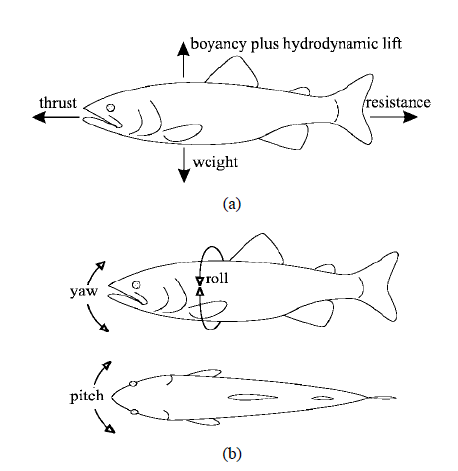
\includegraphics[scale=0.5]{force.png}
    \caption{Forces acting on a swimming fish (a). Dynamics variable definitions (b). Adapted from \citet{magnuson}}
    \label{fig:force}
\end{figure}
Investigation of fish hydrodynamics has led to several findings \citet{lauder1}. It is outlined that fish has several key characteristics in it's locomotion. Fish is statically unstable, which leads to the need of constant active control of fin, even during hovering. Fish fin is also flexible, which enables fish to direct the force generated by the fins and plays a role in thrust generation. This flexibility along with the existence of fin rays make it possible for fish to change it's fin curvature, enabling the fish to resist more hydrodynamic load. It is also observed that fish fins move in a complex three-dimensional manner. Experimental setup usually treated fish fin as undulating model, however the observation that three-dimensional motion is present even in steady locomotion of fish make this treatment inadequate in understanding fish fin function. This three-dimensionality effect leads to the understanding that dorsal and anal fin also contributes as much thrust as the tail. This also leads to the speculation that difference in locomotion patterns of fish is the result of different three-dimensional effect and fin use. However, if fish from different species with different swimming characteristics is observed in it's horizontal section during swimming, it is found that fish swims in similar manner accross species, which leads to the conclusion that 2D patterns of undulation is very similar among fishes.\par
While fish fin motion might seem complex at a glance, usually caudal fin oscillating motion is simplified into pitching and heaving motion only. Figure \ref{fig:caudalfinkinem} illustrate a fish during it's motion.
\begin{figure}[H]
    \centering
    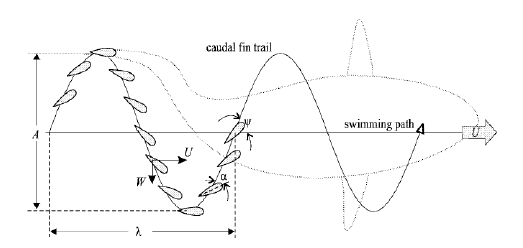
\includegraphics[scale=0.75]{caudalfinkinem.png}
    \caption{Lateral view of caudal fin. Adapted from \citet{magnuson}}
    \label{fig:caudalfinkinem}
\end{figure}
Amplitude $A$ is the maximum width of heaving motion of the fin, wavelength $\lambda$ refers to the length of wave that the fish body mimics as it swims, angle of attack $\alpha$ refers to the angle of the chord line with respect to the caudal fin's trail, feather angle $\Psi$ is the angle between the fin trail and it's swimming path, $U$ and $W$ refers to the swimming velocity parallel and perpendicular to the fish's swimming path, respectively \citep{sfakiotakis}.
\subsection{Derivation of the Flow Equation}
\label{sec:8}
Consider a 3-D flapping body immersed in an incompressible Newtonian fluid. Following \citet{borazjani}, the Navier-Stokes equation that has been non-dimensionalised by characteristic reference velocity $U$ and fin length $L$ can be rewritten as:
\begin{equation}
    \nabla^{*} \cdot \mathbf{u}^{*} = 0
    \label{eq:consofmass}
\end{equation}
\begin{equation}
    \frac{\partial \mathbf{u}^{*}}{\partial t^{*}} + \left(\mathbf{u}^{*} \cdot \nabla^{*} \right) \mathbf{u}^{*} = -\nabla^{*}p^{*} + \frac{1}{Re} \nabla^{*^{2}}\mathbf{u}^{*}
    \label{eq:consofmomentum}
\end{equation}
Equation \ref{eq:consofmass} describe the conservation of mass during the fluid motion, which states that the volume of the fluid element does not change during motion. The right hand terms of equation \ref{eq:consofmomentum}, which is basically the Newton's second law on motion or conservation of momentum, describes the effect of pressure and viscosity on the motion of a fluid. Reynolds number, denoted by $Re$ describes the ratio between inertial effect and viscous dissipation. It can then be inferred that, depending on the swimming condition, as $Re$ becomes higher, the viscous effect of the fluid can be neglected, and vice versa.\par
Rewriting equation \ref{eq:consofmomentum} in terms of vorticity can be more helpful as pressure distribution is more difficult to measure experimentally \citep{dea}. Non-dimensionalised vorticity $\boldsymbol{\omega}^{*}$ is defined as:
\begin{equation}
    \boldsymbol{\omega}^{*} = \nabla^{*} \times \mathbf{u}^{*}
    \label{eq:defineomega}
\end{equation}
Taking the curl of equation \ref{eq:defineomega} and plugging in definition from \ref{eq:consofmomentum} will yield:
\begin{equation}
    \frac{\partial \boldsymbol{\omega}^{*}}{\partial t^{*}} = \nabla^{*} \times \left(\mathbf{u}^{*} \times \boldsymbol{\omega}^{*} \right) + \frac{1}{Re} \nabla^{*^{2}} \boldsymbol{\omega}^{*}
    \label{eq:consofvorticity}
\end{equation}
Equation \ref{eq:consofvorticity} is the same as equation \ref{eq:consofmomentum}, written in terms of non-dimensionalised vorticity $\boldsymbol{\omega}^{*}$.\par
To derive an expression for force generated by a fish fin in mathematical form, thin airfoil theory will be used. Integrate small vorticity element over the surface area $S$ of an airfoil, bounded by closed contour $\Sigma$:
\begin{equation}
    \oint\limits_{\Sigma} \mathbf{u}^{*} \cdot\, \mathrm{d}l^{*} = \iint\limits_{S} \boldsymbol{\omega}^{*} \cdot \mathbf{n}^{*}\, \mathrm{d}S^{*}
    \label{eq:vortintegrate}
\end{equation}
to obtain circulation $\Gamma$. Applying Kutta-Jokowski theorem and adding the circulation term, force can be written in mathematical form as:
\begin{equation}
    \mathbf{F} = -\rho\frac{\mathrm{d}}{\mathrm{d}t} \int\limits_{R} \mathbf{r} \times \boldsymbol{\omega}\, \mathrm{d}R+ \rho\frac{\mathrm{d}}{\mathrm{d}t} \int\limits_{S} \mathbf{v} \cdot \mathbf{n}\, \mathrm{d}A
    \label{eq:forcevort}
\end{equation}
$\mathbf{v}$ is defined as induced velocity, which exist due to the presence of non-zero vorticity $\boldsymbol{\omega}$ of a small fluid element $\mathrm{d}V$ at a distance $\mathbf{r}$ from the region of interest. According to Biot-Savart law, the induced velocity can be expressed as:
\begin{equation}
    \mathbf{v} = \frac{1}{4\pi} \int\limits_{V} \boldsymbol{\omega} \times \frac{\mathbf{r}}{\mathbf{r}^{3}}\, \mathrm{d}V
    \label{eq:biotsavartvelo}
\end{equation}
Equation \ref{eq:forcevort} states that the force acting on an airfoil is generated by the vorticity arisen from the movement of the airfoil, expressed in the first term on the right hand side of the equation and inertial force of the fluid displaced by the airfoil body, shown in the second term of the right hand side of the equation.
\subsection{Scaling Parameters}
\label{sec:9}
The introduction of scaling parameters, combination of multiple parameters into a set of non-dimensional parameters, helps reduce the number and complexity of parameters involved in the experiment \citep{shyy}. There are three common scaling parameters used in caudal fin analysis:
\begin{enumerate}
    \item Reynolds number $Re$: the ratio between fluid inertia and viscous dissipation.
    \begin{equation}
        Re = \frac{U L}{\nu}
    \end{equation}
    where $U$ denotes freestream velocity of the fluid, $L$ signifies reference length, and $\nu$ denotes kinematic viscosity. For scaled objects with identical $Re$, the value of non-dimensional fluid properties and force is the same.
    \item Strouhal number $St$: the ratio of fin flapping frequency to forward swimming speed.
    \begin{equation}
        St = \frac{f A}{U}
    \end{equation}
    where $f$ denotes the flapping frequency, $A$ signifies the width of the wake in lateral direction, and $U$ denotes freestream velocity of the fluid.
    \item Reduced frequency $k$: a scaling parameters similar to Strouhal number, but represents flow unsteadiness better than Strouhal number.
    \begin{equation}
        k = \frac{\pi f L}{U}
    \end{equation}
    where $f$ denotes the flapping frequency, $L$ signifies the length of the fin, and $U$ denotes freestream velocity of the fluid.
\end{enumerate}
\subsection{Hydrodynamics of Caudal Fin}
\label{sec:10}
Thrust generated by undulatory motion is similar to that of thrust generated by propeller, by producing localised thrust wake with an observable momentum jet, as illustrated in figure \ref{fig:vortex}.
\begin{figure}[H]
    \centering
    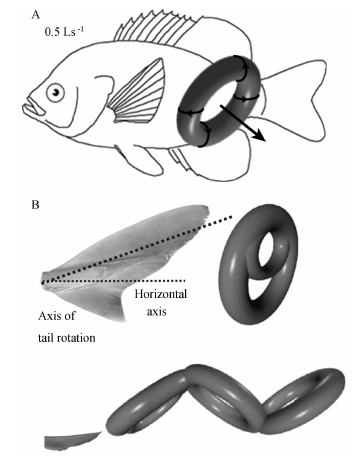
\includegraphics[scale=0.5]{vortex.png}
    \caption{Vortex ring around bluegill sunfish (A) and the tail of leopard sharks (B). Adapted from \cite{lauder1}}
    \label{fig:vortex}
\end{figure}
In the case of fish, thrust is generated by a backward-moving propulsive wave that extends to it's caudal fin \citep{sfakiotakis}. A foil (or in this case, a fin) in steady forward motion combined with steady-state harmonic heaving and pitching motion produces thrust through the formation of a flow downstream from the trailing edge, which when averaged over a period of oscillation has the form of a jet \citep{anderson}. This undulatory motion also generated a large side force that is speculated to be necessary for maintaining stability or simply a consequence of the undulatory motion itself \citep{lauder1}.\par
Particle image velocimetry (PIV) method has shed some light on the behaviour of water around a flapping fin in the recent years by allowing visualisation of water flow around the body of swimming fish. In this method, laser light is focused into a 2D light sheet and images are then obtained from high-speed videos of particles moving with the flow, which gives detailed time-dependent description of water flow patterns, calculation of wake vorticity and estimation of force. This 2D PIV approach has been extended into volumetric 3D imaging capability, which provides instantaneous 3D flow reconstructions of the wake produced by the fish' body and fins during swimming \citep{lauder2}.\par
Caudal fin produced wake consisted of a series of string counter-rotating vortices, typical of structure of a series of linked in vortex rings as shown in figures \ref{fig:wake1} and \ref{fig:wake2}. Between each pair of counter-rotating vortices, a jet of high velocity of flow was formed \citep{nauen}.\par
\begin{figure}[H]
    \centering
    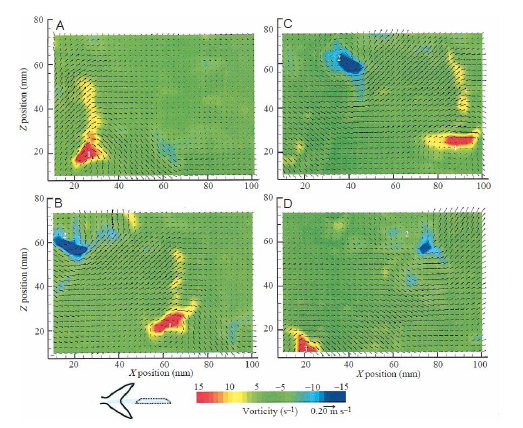
\includegraphics[scale=0.75]{wakepiv1.png}
    \caption{The time course of vortex production over approximately one tail beat of a Scomber japonicus 24 cm in fork length (FL) swimming at 1.2 FL s–1. The distal tips of the caudal fin were positioned approximately 1 cm to the left of the flow fields shown. The caudal fin was moving through the horizontal (XZ) light sheet at the position of the fin’s lateral. Flow velocity is represented by the black vectors plotted over a color background indicating flow vorticity. Vortices in the wake are numbered consecutively in the order in which they are shed from the caudal fin. Adapted from \citet{nauen}}
    \label{fig:wake1}
\end{figure}
\begin{figure}[H]
    \centering
    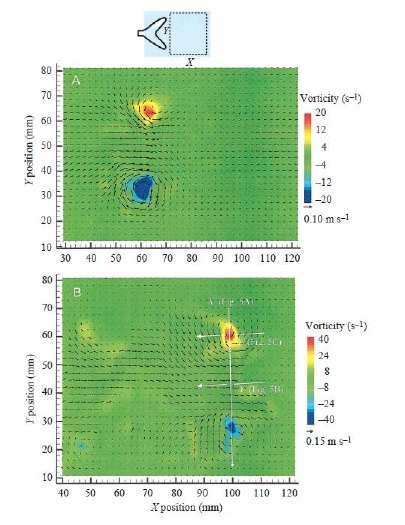
\includegraphics[scale=0.75]{wakepiv2.png}
    \caption{Views if the wake in the vertical (XY) plane of an individual of Scomber japonicus 26 cm in fork length swimming steadily at speeds of 1.2 \textit{FL s}\textsuperscript{-1} (A) and 2.2 \textit{FL s}\textsuperscript{-1}, where \textit{FL} is the fork length (B). Flow velocity is represented by black vectirs plotted over a color background indicating vorticity. At both swimming speeds, the caudal fin sheds one pair of counter-rotating vortices with central jet of high velocity per stroke.}
    \label{fig:wake2}
\end{figure}
\begin{figure}[H]
    \centering
    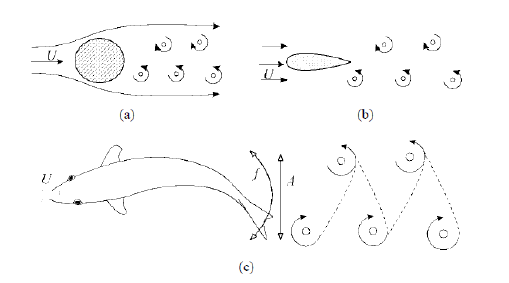
\includegraphics[scale=0.75]{karmanstreet.png}
    \caption{The Karman street generates a drag force for either (a) bluff or (b) streamlined bodies, placed in a free stream. (c) The wake of swimming fish has reverse rotational direction, associated with thrust generation.}
    \label{fig:karmanstreet}
\end{figure}
As caudal fin moves back and forth, the wake left behind the tail of undulatory swimmer is a staggered array of trailing discrete vortices of alternating sign as shown in figure \ref{fig:karmanstreet}. This reversed rotational direction produced thrust instead of drag that is produced by the well-documented Karman vortex sheet. This propulsive wave traverse the fish body in opposite direction to the fish' overall movement and faster that the overall swimming speed \citep{sfakiotakis}.
\section{Fundamentals of Global Surrogate Assisted Genetic Algorithm}
\label{sec:11}
This subsection will explain the fundamentals of genetic algorithm used for optimisation process. The fundamentals of single objective genetic algorithm will be explained in \ref{sec:12}, the concept of surrogate modeling and it's construction with Kriging method will be explained in \ref{sec:13}, and the coupling between GA and surrogate modeling will be outlined in \ref{sec:14}.
\subsection{Fundamentals of Single-Objective Genetic Algorithm}
\label{sec:12}
Optimisation is defined as the process of adjusting a set of input variables to a mathematical process or function i.e fitness function in order to find maximum or minimum output or result i.e fitness \citep{haupt}. There are many approaches to optimise a function, among them are analytical optimisation and natural optimisation. Analytical optimisation is based on the idea that the optimum of a function is reached when the first derivative of a function is equal to zero. This begs the question: what if the function is not explicit? Or continuous? What if the fitness is a function of many variables? Realising that many cases in real-life cannot be modeled in a straightforward manner renders analytical optimisation impractical. Natural optimisation approach is different from analytical approach in a sense that instead of finding the fitness function to obtain fitness, natural optimisation moves intelligently from point to point in a predefined search space to obtain fitness, or in simple terms ``intelligent trial-and-error''. One such approach is called genetic algorithm (GA) which is based on principle of genetics and natural selection.\par
In GA, a set of variables is treated as a population composed of single individuals which is allowed to evolve according to the principles of genetic recombination and natural selection under  a set of selection rules to obtain fitness value. GA was first developed by John Holland and David Goldberg in the 70s to solve gas-pipeline transmission control problem. GA is further divided based on the amount of objectives into single-objective where the fitness of a single fitness function and multi-objective where one evaluates the fitness(es) of several fitness functions from similar input. How the input of a variable is formulated also differs GA: binary GA, where the input is represented as a string of encoded binary numbers, which is simple and similar to how chromosomes work in nature but also unsuitable for continous, multi-variable or high-precision problems; and real GA (RGA) where each individual is represented with floating-point numbers \citep{haupt}.\par
\begin{figure}[H]
    \centering
    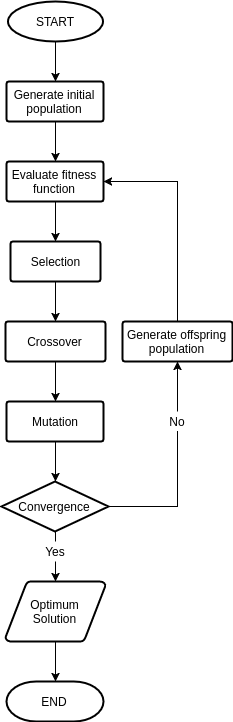
\includegraphics[scale=0.7]{flowchartrga.png}
    \caption{Flowchart of basic real single-objective genetic algorithm.}
    \label{fig:flowchartrga}
\end{figure}
Flowchart shown in figure \ref{fig:flowchartrga} shows that the process of RGA to find the fitness value of fitness function $f(\mathbf{x})$ with input $\mathbf{x} = [\mathbf{x}^{(1)}, \mathbf{x}^{(2)}, \ldots, \mathbf{x}^{(N)}]^{T}$ can be divided into five steps which consists of:
\begin{enumerate}
    \item Initial population generation

    GA begins with generating random $N_{pop} \times N_{var}$, where $N_{var}$ is the number of variables and $N_{pop}$ is the number of individuals inside the population on each generation. All variables are normalised into real numbers $x_{norm}$ between $[0, 1]$ convenience sake. Unnormalised variable $x$ is obtained from the following equation:
    \begin{equation}
        x = x_{l} + \left(x_{h} - x_{l}\right)x_{norm}
        \label{eq:norm2unnorm}
    \end{equation}
    where $x_{l}$ and $x_{h}$ are the lowest and highest number in the variable range, respectively.
    \item Fitness function evaluation

    Individuals are then evaluated using a known fitness function $f(\mathbf{x})$. If $f(\mathbf{x})$ is unknown, then each individual in the population is evaluated through either numerical simulation or experiment.
    \item Selection

    Population are selected in a similar way to Darwinian natural selection to form a mating pool. There are several methods to perform selection such as top-to-bottom, random, weighted, cost and tournament pairing. Tournament selection method is used for selection method in this thesis. In this approach, two individuals are randomly selected from the population and undergoes mating competition where the individual with lower fitness wins (i.e enter the mating pool). This process will produce a $N_{pop} \times N_{var}$ mating pool matrix for crossover process \citep{haupt}.
    \item Crossover

    Crossover is the analogy to reproduction in real-life evolution process where two individuals ``marry off'' to create a new individual i.e an offspring. The method for crossover used in this thesis is simulated binary crossover (SBX). SBX is an adaptive search method where the crossover probability of distribution depends on how close an offspring is to it's parents. As the solution converges, the offspring becomes more similar to it's parents \citep{deb}.
    \item Mutation

    Just like it's natural counterpart, mutation in GA is an alteration introduced to the offsprings that occurs constantly according to a small mutation probability. In GA process, mutation prevents the solution from converging too quickly at a local optimum.
\end{enumerate}
\subsection{Global Surrogate-Assisted Genetic Algorithm (G-SAGA)}
\label{sec:13}
From \ref{sec:12} it is implied that the larger the population, the more robust the optimisation. Consider now a population consisting of 100 individuals and GA iteration that loops until 100 generation. This means that one have to do 10000 experimental or numerical runs, which is expensive. To overcome this problem, a surrogate model was used in this thesis. Surrogate models are models that are built to approximate the ``true'' fitness function $f(\mathbf{x})$ to decrease computational or experimental cost massively. It also provides insight on how an input $\mathbf{x}$ affects the output $\mathbf{y}$ (\cite{ong}). If a case is represented mathematically as:
\begin{equation}
    y = f(\mathbf{x})
    \label{eq:truefcn}
\end{equation}
then the surrogate model is an approximation of the form
\begin{equation}
    \hat{y} = \hat{f}(\mathbf{x})
    \label{eq:approxfcn}
\end{equation}
such that
\begin{equation}
    y = \hat{y} + \epsilon
    \label{eq:true2approx}
\end{equation}
It can then be inferred that, in a sense, surrogate modeling process is a surface fitting process that mimics the real behaviour of a physical process. In this thesis, Kriging was chosen to be the surrogate modeling method.\par
\begin{figure}[H]
    \centering
    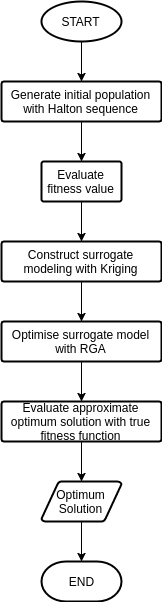
\includegraphics[scale=0.7]{flowchartkrig.png}
    \caption{Flowchart of surrogate-assisted genetic algorithm.}
    \label{fig:flowchartkrig}
\end{figure}
Figure \ref{fig:flowchartkrig} illustrated the flowchart of surrogate-assisted genetic algorithm. As with basic GA, G-SAGA begins with population generation $N_{pop}$. This population was generated using a sampling plan algorithm called Halton sequence \citep{bimo}. Each individuals of $N$ amount are then evaluated through experiment to obtain responses $\mathbf{y} = [y^{(1)}, y^{(2)}, \ldots, y^{(N)}]^{T}$ that correlates to sample set $\mathbf{x} = [\mathbf{x}^{(1)}, \mathbf{x}^{(2)}, \ldots, \mathbf{x}^{(N)}]^{T}$. The evaluation result is then fitted using Kriging to obtain the surrogate model $\hat{f}(\mathbf{x})$ that approximate the true fitness function $f(\mathbf{x})$. Approximate optimum solution $\mathbf{x}_{opt}$ was obtained by optimising the surrogate model $\hat{f}(\mathbf{x})$ using RGA. This approximate optimum solution $\mathbf{x}_{opt}$ is finally evaluated using experiment to generate the best fitness value $y_{opt} = f(\mathbf{x}_{opt})$. Using this approach, instead of having to do 10000 times experimental runs to obtain an optimum solution, one only have to do 100 experimental runs to obtain the initial correlation between $y$ and $\mathbf{x}$ and run one more experiment on the optimum solution $\mathbf{x}_{opt}$, reducing the workload up to 99\%. This thesis used G-SAGA code created by \citet{bimo} for single objective case with few modifications to connect the algorithm to the experimental system.
\subsection{Fundamentals of Kriging}
\label{sec:14}
Kriging is defined as design and analysis of computer experiments model \citep{sacks} or Gaussian process regression \citep{williams}. One may think of it as a n-dimensional curve or surface fitting method.\par
Given a set of $n$ noise-free sample data, $\mathbf{x} = [\mathbf{x}^{(1)}, \mathbf{x}^{(2)}, \ldots, \mathbf{x}^{(n)}]^{T}$ that correlates to response $\mathbf{y} = [y^{(1)}, y^{(2)}, \ldots, y^{(n)}]^{T}$. The relation between sample set and responses is denoted using a set of vectors
\begin{equation}
    \mathbf{Y} =
        \begin{bmatrix}
            Y(\mathbf{x}^{(1)}) \\
            Y(\mathbf{x}^{(2)}) \\
            \vdots \\
            Y(\mathbf{x}^{(n)})
        \end{bmatrix}
    \label{eq:set2resp}
\end{equation}
Each elements in vector $\mathbf{Y}$ are connected with each other with a basis function
\begin{equation}
    \mathrm{cor}[Y(\mathbf{x}^{(i)}),Y(\mathbf{x}^{(l)})] = \exp\left(-\sum_{j=1}^{k}\boldsymbol{\theta}_{j}\lvert x_{j}^{(i)} - x_{j}^{(l)}\rvert^{\mathbf{p}_{j}}\right)
    \label{eq:basisfcn2cor}
\end{equation}
\par
The right hand side term of equation \ref{eq:basisfcn2cor} is a basis function for a surrogate model construction called Kriging. In kriging, the basis function $\psi$ is expressed as:
\begin{equation}
    \psi^{(t)} = \exp\left(-\sum_{j=1}^{k}\boldsymbol{\theta}_{j}\lvert x_{j}^{(i)} - x_{j}^{(l)}\rvert^{\mathbf{p}_{j}}\right)
    \label{eq:basiskriging}
\end{equation}
Equation \ref{eq:basiskriging} basically gives the basis needed to construct the Kriging model by solving for $\boldsymbol{\theta}$ and $\mathbf{p}_{j}$, where $\boldsymbol{\theta} = [\theta_{1}, \theta_{2}, \dots, \theta_{k}]^{T}$ is the basis vector (similar to $\hat{i}$, $\hat{j}$, and $\hat{k}$ in Cartesian basis) and $\mathbf{p}_{j} = [p_{1}, p_{2}, \dots, p_{k}]^{T},\, \mathbf{p}_{j}\in[1,2]$ is the exponent vector.\par
The construction of surrogate model with Kriging starts with maximisation of likelihood function $L$, expressed in natural logarithmic $\ln$ as
\begin{equation}
    \ln L = -\left(\frac{n}{2}\ln(2\pi) + \frac{n}{2}\ln(\sigma^{2}) + \frac{1}{2}\ln\lvert\boldsymbol{\Psi}\rvert + \frac{\left(\mathbf{y} - \mathbf{1}\mu\right)\boldsymbol{\Psi}^{-1}\left(\mathbf{y} - \mathbf{1}\mu\right)}{\sigma^{2}}\right)
    \label{eq:likelihoodfcn}
\end{equation}
where $\sigma^{2}$ is the variance, $\mathbf{1}\mu$ is the mean of random vector $\mathbf{Y}$, and $\mathbf{1}$ is an $1 \times n$ column vector consisting of ones. $\boldsymbol{\Psi}$ is Gram matrix defined as
\begin{equation}
    \boldsymbol{\Psi} =
        \begin{bmatrix}
            \mathrm{cor}[Y(\mathbf{x}^{(1)}),Y(\mathbf{x}^{(l)})] & \dots & \mathrm{cor}[Y(\mathbf{x}^{(1)}),Y(\mathbf{x}^{(n)})] \\
            \vdots & \ddots & \vdots \\
            \mathrm{cor}[Y(\mathbf{x}^{(n)}),Y(\mathbf{x}^{(l)})] & \dots & \mathrm{cor}[Y(\mathbf{x}^{(n)}),Y(\mathbf{x}^{(n)})]
        \end{bmatrix}
    \label{eq:grammat}
\end{equation}
by deriving equation \ref{eq:likelihoodfcn} once and equating it with zero, maximum likelihood estimates (MLEs) for variables $\sigma^{2}$ and $\mu$ is obtained
\begin{equation} \label{eq:sigmamu}
\begin{split}
    \hat{\mu} &= \frac{\mathbf{1}^{T}\boldsymbol{\Psi}^{-1}\mathbf{y}}{\mathbf{1}^{T}\boldsymbol{\Psi}^{-1}\mathbf{1}} \\
    \hat{\sigma}^{2} &= \frac{\left(\mathbf{y} - \mathbf{1}\mu\right)^{T}\boldsymbol{\Psi}^{-1}\left(\mathbf{y} - \mathbf{1}\mu\right)}{n}
\end{split}
\end{equation}
substituting equation \ref{eq:sigmamu} to \ref{eq:likelihoodfcn} and removing constant terms from the same equation, a simplified function called the ``concentration $\ln$-likelihood function'' is obtained
\begin{equation}
    \ln(L) \approx -\left(\frac{n}{2}\ln(\sigma^{2}) + \frac{1}{2}\lvert\boldsymbol{\Psi}\rvert\right)
    \label{eq:conclikelihood}
\end{equation}
following \citet{forrester}, by deriving likelihood function $L$, the surrogate model $\hat{f}(\mathbf{x})$ of a fitness function $f(\mathbf{x})$ is
\begin{equation}
    \hat{f}(\mathbf{x}) = \hat{\mu} + \boldsymbol{\psi}^{T}\boldsymbol{\Psi}^{-1}\left(\mathbf{y} - \mathbf{1}\hat{\mu}\right)
    \label{eq:surrogatefcn}
\end{equation}
where $\boldsymbol{\psi} = [\psi^{(1)}, \psi^{(2)}, \dots, \psi^{(n)}]^{T}$ is the basis function vector. Equation \ref{eq:surrogatefcn} shows that surrogate model $\hat{f}(\mathbf{x})$ is a function of basis vector $\boldsymbol{\theta}$ and exponent vector $\mathbf{p}_{j}$ inside $\boldsymbol{\psi}$ and $\boldsymbol{\Psi}$. This method is called Kriging interpolation.\par
Recall that Kriging interpolation that is derived previously assumes that the sample set is noise-free. However, there exist random noise during force measurement in towing tank experiment during fitness evaluation. To filter noisy sample data, a regression constant $\lambda$ is introduced into equation \ref{eq:surrogatefcn} so that it becomes
\begin{equation}
    \hat{f}(\mathbf{x}) = \hat{\mu}_{r} + \boldsymbol{\psi}^{T}\left(\boldsymbol{\Psi} + \lambda\mathbf{I}\right)^{-1}\left(\mathbf{y} - \mathbf{1}\hat{\mu}_{r}\right)
    \label{eq:surrogatefcnmod}
\end{equation}
where
\begin{equation}
    \hat{\mu}_{r} = \frac{\mathbf{1}^{T}(\boldsymbol{\Psi} + \lambda\mathbf{I})^{-1}\mathbf{y}}{\mathbf{1}^{T}(\boldsymbol{\Psi} + \lambda\mathbf{I})^{-1}\mathbf{1}}
    \label{eq:mur}
\end{equation}
\par
In this thesis, the exponent vector was set to a constant value $\mathbf{p}_{j} = 2$, while the basis vector $\boldsymbol{\theta}$ was set in the range $\boldsymbol{\theta}\in[10^{-3},10^{2}]$. The value of regression constant $\lambda$ was set in the range $\lambda\in[10^{-6},1]$.\par